\section{PyTorchGUI}
\subsection{Functional design}

The main goal of the project is to create a graphical interface which will allow to manipulate the different features of PyTorch. By observing the way Expresso works for Caffe, and what PyTorch allows the user to do, we listed the different features that could be interesting for our application :
We have decide to spread the functionality between multiple tabs to simplify the interface of the application.

We decided to divide our application in four different parts, which are directly inherited from what has been done in Expresso.

The first one, data view, gives a way for the user to import and edit data which will be used in other parts by creating data sets.

The second one, network view, allows the user to configure the neural networks which will be used for the training.

The third one, Train View allow to to train a neural network, by using the data training set

Finally, the experiment view can allow diverse operations, such as visualizing network features, and evaluating a trained network

Here are the different specifications for each of these parts. Some of them are optional, and will be developed if we have the time.

\begin{itemize}
   \item Data View Tab
   \begin{itemize}
     \item Allowing different types of data : the application needs to allow the import of image files such as jpeg and png, but we can extend this to other data files types (hdf5,csv).
     A hdf5 is a container, in our case it will contains pictures.
     
     The csv file contains annotations for pictures (like coordinates that we must use for face delimitation for example).
     
     The application should at least read png, jpeg and csv files. The rest is optional.
     
     \item  By opening a window, the app can allow to choose a particular file from a directory. We must verify that the open file is a supported file (in the list above), that it opens correctly, if not we must notify it to the user.
     \item The user can give a name to a set of data, it must be a name that is not used for the moment. If not we must notify it to the user.
     \item The app can allow to visualize an imported image, if it's a hdf5 file we must visualize one image by one image.
     \item Operations on data : The user can split data in different sets, by choosing the percentage of each part (it will be useful if the user doesn't want to train all the data with the same model). He can also generate random data, by choosing a range. Once imported and modified, data can also be exported. Annotations can also be added to data, and variables can be renamed.
     \item To facilitate visualization, data is separated by color
   \end{itemize}
   \pagebreak
   \item Network View Tab
   \begin{itemize}
         \item The user will be able to construct the net from scratch.
         \item The user can add a layer, edit a layer (he can modify its parameters), and delete a layer.
         \item The user can visualise the layers of the network architecture.
         \item The user can save the net configuration, and he can import another configuration. (in a configuration file, which works like prototxt files in Caffe)
         \item The user can choose to use GPU instead of CPU for computation. Indeed, if the user has a GPU with enough performance, computation will be quicker by using its capacity instead of the CPU.
     
   \end{itemize}
   \item Train View Tab
   \begin{itemize}
   \item In this Tab users can edit the training parameters.
    \begin{itemize}
        \item The number of Iteration (Total number of forward passes a test has to carry out).
        \item Test Interval (Total number of training iterations, after which Testing is conducted).
        \item Lr( Learning rate: it is how quickly a network abandons old beliefs for new ones)
        \item Momentum (it is a value between 0 and 1 that increases the size of the steps taken towards the minimum by trying to jump from a local minima).
        \item Weight Decay of the network
        \item Display (Display contains values of iterations after which current state is displayed).
        \item Max Iteration (It is the upper limit for training iterations).
        \item Snapshot (The interval after which intermediate parameters are stored).
    \end{itemize}
    Then the user must have to validate the parameters to access to the next Tab by clicking on a Next button.
    \item Training dataset : the user chooses the data to train. (He can choose into a list of all data-sets that were created or loaded before)
    \item Next, the user will be able to edit the training batch size (the number of training examples utilized in one iteration).
    \item Users can choose a name of Trained Model.
    \item Some operations can take a long time (a few minutes or even hours) and requires the app to give feedback to the user. To do so we can display a progress bar when importing a file, and when computing data.  Alternatively, we can let a task run in the background, and notify the user once it's done. (optional)
    
    Users have to validate the parameters by clicking on a Finish button.
   \end{itemize}
   
   \item Experiment View Tab
   
   Once the calculation are completed users will access to a Visualize Tab, where they will be able to visualize  the resulting pictures.
   \begin{itemize}
       \item Extract features via pre-trained Net (optional)
       \begin{itemize}
           \item Selection of the Deploy net, the users will check which layer(s) he wants to use(exemple: relu, conv2, conv1).
           \item Users will have to select the data that they want to use.
           \item The user can choose the name of the variable that will be generated
       \end{itemize}
   \end{itemize}
   Once the data extracted users can display the results. These results are a colorized version of the input image, which shows clearly the patterns (example available in Annexes - "Expresso Experimental View (Visualise features)
   
   \begin{itemize}
   \item Users will have the possibility to display graphics representing the accuracy, and the loss over the training. This is the evaluating part. The application has to at least display the accuracy, the rest is optional.
   \item Users will be able to save their results and choose a name to their file.
   
   \end{itemize}
   
\end{itemize}



The application must also be able to keep everything that has been opened or calculated in memory as long as we do not delete the data of the application or until we close it.

\begin{figure}[!ht]
\center
    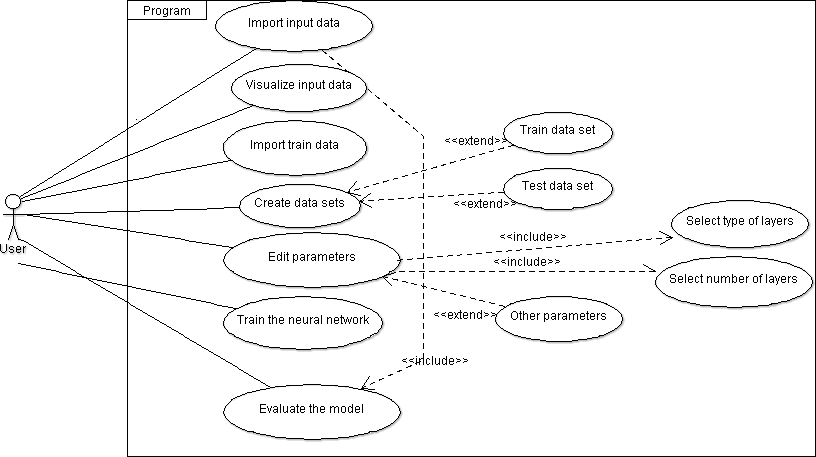
\includegraphics[scale=0.6]{figures/useCase2.png}
    \caption{Use cases diagram}
\end{figure}

\subsection{Non-functional design}

\subsection{Constraints}

\begin{itemize}
\item Platform-compatibility : The app has to be compatible with Linux. If possible, we will try to make it work also with other platforms.
\item Maintainability : We have to develop our application in a way that allows future developers to extend the functionalities. Also, we have to make sure that our app will easily be compatible with future versions of PyTorch.
\end{itemize}

\subsection{Choice of application type}

To develop our application we were thinking about two types of applications. These two choices are a Web-Service, or a regular application.
In order to choose which type of application to develop we drew up a table of advantages and disadvantages.

\begin{itemize}
    \item Web-Service advantages :
    \begin{itemize}
         \item The Web application can be used by all users anywhere and when they want if they are connected to Internet. Furthermore, this facilitates a simple to get a multi-platform application.
        \item The application is always up to date, if it needs an update we only have to update the server whereas a simple application have to be updated on all users' computer. The app is more flexible.
        \item The deployment of the app is easier
        \item It could facilitate the extension of the app to add features
    \end{itemize}
\end{itemize}

 
 \begin{itemize}
    \item Web-Service drawbacks :
    \begin{itemize}
         \item Users need to be connected and to have good network performance (fast and stable) especially in case of big data exchanges. In addition, the server could have to support many users at the same time. Even if the app is running in local, they need to have a good central server, which needs a more complex architecture.
        \item With the same hardware, performances are lower than a native application, we have to exchange data with the server so it must take a long time before getting results especially if we have a lot of data in addition of the time of calculation.
        \item Complex visual effects like drawing a graph could be more complicated to implement
        
    \end{itemize}
\end{itemize}

  \begin{itemize}
    \item Native Application advantages :
    \begin{itemize}
        \item Users don't need an Internet connection.
        \item It has got better performances, better time of calculation, better time of response.(Faster than a Web-Service)
    \end{itemize}
\end{itemize}
\begin{itemize}
    \item Native Application disadvantages :
    \begin{itemize}
        \item Every user have to install the application on his personal computer.
         \item If the application needs an update, we have to upgrade all the computers equipped with the application.
    \end{itemize}
\end{itemize}

\textbf{Our choice :}
Since both options seemed quite equivalent for us, and since having a web-service deployment wasn't a need for the project, we decided to go on to the \textbf{Native Application}. Indeed, this will perfectly allow us to implement all needed features with performance similar to those of PyTorch by itself.

\subsection{Tests}
To make sure the application is working properly, we need to test all features with determined data sets.

Examples of tests :
\begin{itemize}
\item Importing an image and visualise it
\item Importing a set of data, edit its variables and export it
\item Importing a training file, visualize the layers, add a layer, modify a layer, delete a layer, and saving the configuration
\item Testing that the results of classification are always the same as when we use PyTorch in console mode
\item Ergonomics and stability : we have to test that all buttons do an action, that they do the right action, that the application does not crash, and that it is well integrated to the operating system
\end{itemize}
\begin{itemize}
\item In a general way, our tests will consist of being able to use all of PyTorch features with our application, by using default PyTorch test sets.
\end{itemize}

\section{Jupyter NoteBook}
\pagebreak